\documentclass[dvipdfmx]{jsarticle}

\title{ブロック落しゲーム(JavaScript)}
\author{Seiichi Nukayama}
\date{2020-06-21}
\usepackage{tcolorbox}
\usepackage{color}
\usepackage{listings, plistings}

% Java
\lstset{% 
  frame=single,
  backgroundcolor={\color[gray]{.9}},
  stringstyle={\ttfamily \color[rgb]{0,0,1}},
  commentstyle={\itshape \color[cmyk]{1,0,1,0}},
  identifierstyle={\ttfamily}, 
  keywordstyle={\ttfamily \color[cmyk]{0,1,0,0}},
  basicstyle={\ttfamily},
  breaklines=true,
  xleftmargin=0zw,
  xrightmargin=0zw,
  framerule=.2pt,
  columns=[l]{fullflexible},
  numbers=left,
  stepnumber=1,
  numberstyle={\scriptsize},
  numbersep=1em,
  language={Java},
  lineskip=-0.5zw,
  morecomment={[s][{\color[cmyk]{1,0,0,0}}]{/**}{*/}},
}
%\usepackage[dvipdfmx]{graphicx}
\usepackage{url}
\usepackage[dvipdfmx]{hyperref}
\usepackage{amsmath, amssymb}
\usepackage{itembkbx}
\usepackage{eclbkbox}	% required for `\breakbox' (yatex added)
\usepackage{setspace}
\usepackage{multicol}
\fboxrule=1pt
\parindent=1em
\begin{document}

%% 修正時刻: Sun Jun 21 08:35:35 2020


\section{ブロックの種類を増やして、上下キーに割り当てる}

ブロックの種類を増やします。多次元配列を使います。\\
以下のように block変数を書き換えてください。

\begin{lstlisting}
  const block = [
    [      // block0 -- 凸型
      [
        [0, 0, 0, 0],
        [1, 1, 1, 0],
        [0, 1, 0, 0],
        [0, 0, 0, 0]
      ],
      [
        [0, 1, 0, 0],
        [0, 1, 1, 0],
        [0, 1, 0, 0],
        [0, 0, 0, 0]
      ],
      [
        [0, 1, 0, 0],
        [1, 1, 1, 0],
        [0, 0, 0, 0],
        [0, 0, 0, 0]
      ],
      [
        [0, 1, 0, 0],
        [1, 1, 0, 0],
        [0, 1, 0, 0],
        [0, 0, 0, 0]
      ],
    ],
    [      // block1 -- L型
      [
        [0, 0, 0, 0],
        [1, 1, 1, 0],
        [1, 0, 0, 0],
        [0, 0, 0, 0]
      ],
      [
        [1, 0, 0, 0],
        [1, 0, 0, 0],
        [1, 1, 0, 0],
        [0, 0, 0, 0]
      ],
      [
        [0, 0, 0, 0],
        [0, 0, 1, 0],
        [1, 1, 1, 0],
        [0, 0, 0, 0]
      ],
      [
        [1, 1, 0, 0],
        [0, 1, 0, 0],
        [0, 1, 0, 0],
        [0, 0, 0, 0]
      ],
    ],
    [      // block2 -- 平行四辺形
      [
        [0, 0, 0, 0],
        [0, 1, 1, 0],
        [1, 1, 0, 0],
        [0, 0, 0, 0]
      ],
      [
        [1, 0, 0, 0],
        [1, 1, 0, 0],
        [0, 1, 0, 0],
        [0, 0, 0, 0]
      ],
      [
        [0, 0, 0, 0],
        [0, 1, 1, 0],
        [1, 1, 0, 0],
        [0, 0, 0, 0]
      ],
      [
        [1, 0, 0, 0],
        [1, 1, 0, 0],
        [0, 1, 0, 0],
        [0, 0, 0, 0]
      ],
    ],
    [      // block3 -- 逆L型
      [
        [1, 1, 1, 0],
        [0, 0, 1, 0],
        [0, 0, 0, 0],
        [0, 0, 0, 0]
      ],
      [
        [1, 1, 0, 0],
        [1, 0, 0, 0],
        [1, 0, 0, 0],
        [0, 0, 0, 0]
      ],
      [
        [0, 0, 0, 0],
        [1, 0, 0, 0],
        [1, 1, 1, 0],
        [0, 0, 0, 0]
      ],
      [
        [0, 1, 0, 0],
        [0, 1, 0, 0],
        [1, 1, 0, 0],
        [0, 0, 0, 0]
      ],
    ],
    [      // block4 -- 棒型
      [
        [0, 0, 0, 0],
        [1, 1, 1, 1],
        [0, 0, 0, 0],
        [0, 0, 0, 0]
      ],
      [
        [0, 0, 1, 0],
        [0, 0, 1, 0],
        [0, 0, 1, 0],
        [0, 0, 1, 0]
      ],
      [
        [0, 0, 0, 0],
        [1, 1, 1, 1],
        [0, 0, 0, 0],
        [0, 0, 0, 0]
      ],
      [
        [0, 0, 1, 0],
        [0, 0, 1, 0],
        [0, 0, 1, 0],
        [0, 0, 1, 0]
      ],
    ],
    [      // block5 -- 正方形型
      [
        [0, 0, 0, 0],
        [0, 1, 1, 0],
        [0, 1, 1, 0],
        [0, 0, 0, 0]
      ],
      [
        [0, 0, 0, 0],
        [0, 1, 1, 0],
        [0, 1, 1, 0],
        [0, 0, 0, 0]
      ],
      [
        [0, 0, 0, 0],
        [0, 1, 1, 0],
        [0, 1, 1, 0],
        [0, 0, 0, 0]
      ],
      [
        [0, 0, 0, 0],
        [0, 1, 1, 0],
        [0, 1, 1, 0],
        [0, 0, 0, 0]
      ],
    ],
    [      // block6 -- 逆平行四辺形型
      [
        [0, 0, 0, 0],
        [1, 1, 0, 0],
        [0, 1, 1, 0],
        [0, 0, 0, 0]
      ],
      [
        [0, 1, 0, 0],
        [1, 1, 0, 0],
        [1, 0, 0, 0],
        [0, 0, 0, 0]
      ],
      [
        [0, 0, 0, 0],
        [1, 1, 0, 0],
        [0, 1, 1, 0],
        [0, 0, 0, 0]
      ],
      [
        [0, 1, 0, 0],
        [1, 1, 0, 0],
        [1, 0, 0, 0],
        [0, 0, 0, 0]
      ],
    ]
  ];
\end{lstlisting}

この多次元配列は、たとえば以下のようになります。

\begin{multicols}{3}
 \begin{tcolorbox}
  \textbf{block[0][0]}
\begin{verbatim}
  [0, 0, 0, 0], 
  [1, 1, 1, 0], 
  [0, 1, 0, 0], 
  [0, 0, 0, 0]  
\end{verbatim}
  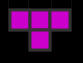
\includegraphics{block0.png}
 \end{tcolorbox}

 \begin{tcolorbox}
  \textbf{block[0][1]}
\begin{verbatim}
  [0, 1, 0, 0],
  [0, 1, 1, 0],
  [0, 1, 0, 0],
  [0, 0, 0, 0]
\end{verbatim}
  
\includegraphics[height=2cm]{block0-1.png}
 \end{tcolorbox}
\end{multicols}

\newpage

\begin{multicols}{3}
 \begin{tcolorbox}
  \textbf{block[1][0]}
\begin{verbatim}
  [0, 0, 0, 0],
  [1, 1, 1, 0],
  [1, 0, 0, 0],
  [0, 0, 0, 0]
\end{verbatim}
  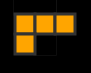
\includegraphics{block1.png}
 \end{tcolorbox}


 \begin{tcolorbox}
  \textbf{block[2][0]}
\begin{verbatim}
  [0, 0, 0, 0],
  [0, 1, 1, 0],
  [1, 1, 0, 0],
  [0, 0, 0, 0]
\end{verbatim}
  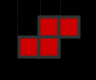
\includegraphics{block2.png}
 \end{tcolorbox}

 \begin{tcolorbox}
  \textbf{block[3][0]}
\begin{verbatim}
  [1, 1, 1, 0],
  [0, 0, 1, 0],
  [0, 0, 0, 0],
  [0, 0, 0, 0]
\end{verbatim}
  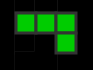
\includegraphics{block3.png}
 \end{tcolorbox}
\end{multicols}

\begin{multicols}{3}
 \begin{tcolorbox}
  \textbf{block[4][0]}
\begin{verbatim}
  [0, 0, 0, 0],
  [1, 1, 1, 1],
  [0, 0, 0, 0],
  [0, 0, 0, 0]
\end{verbatim}
  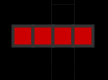
\includegraphics{block4.png}
 \end{tcolorbox}

 \begin{tcolorbox}
  \textbf{block[5][0]}
\begin{verbatim}
  [0, 0, 0, 0],
  [0, 1, 1, 0],
  [0, 1, 1, 0],
  [0, 0, 0, 0]
\end{verbatim}
  
\includegraphics{block5.png}
 \end{tcolorbox}

 \begin{tcolorbox}
  \textbf{block[6][0]}
\begin{verbatim}
  [0, 0, 0, 0],
  [1, 1, 0, 0],
  [0, 1, 1, 0],
  [0, 0, 0, 0]
\end{verbatim}
  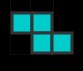
\includegraphics{block6.png}
 \end{tcolorbox}
\end{multicols}

\textbf{block[A][B]} という配列で7種類のブロックを指定できます。\\
\textbf{[A]} でブロックの種類を指定できます。\\
\textbf{[B]} でブロックの向きを指定できます。

これをブロックを描く処理と消す処理に盛り込みます。

また、ブロックの色も7種類作って描く際に選択できるようにします。
ブロックの種類 0...6 に応じて選択します。

先ほどの var block = [ ... ]; の後に以下のコードを付け加えてください。

\begin{lstlisting}
// ブロックの色
const bcolor = ['#CC00CC', '#FFA500', '#CC0000',
        '#00CC00', '#CC0000', '#CCCC00', '#00CCCC']; 
\end{lstlisting}

block[0][?] なら bcolor[0]、block[1][?] なら bcolor[1] となります。

まず、ブロックの種類とその向きを表す変数を設定しておきます。\\

\begin{verbatim}
let col; 
let row;    
\end{verbatim}
の後に記述してください。

\begin{lstlisting}
 let syurui;   // ブロックの種類
 let muki;     // ブロックの向き
\end{lstlisting}

そして、ゲームスタート時にrandom()関数でブロックの種類と向きを選択するよ
うにします。

\begin{lstlisting}
 function gamekaishi() {
   ... (省略) ...
 
   col = 4;
   row = 0;

   syurui = Math.floor(Math.random() * 7);
   muki = Math.floor(Math.random() * 4);;

   kaku(cg, col, row, syurui, muki);
}
\end{lstlisting}

では、「ブロックを描く処理」から修正します。

\begin{lstlisting}
/**
 * ブロックを描く
 * 引数: cv -- canvas
 *        x -- ブロックを描くx座標
 *        y -- ブロックを描くy座標
 *   syurui -- ブロックの種類。0...6 の7種類。
 *     muki -- ブロックの向き。0...3 の3種類。
 */
 function kaku(cv, x, y, syurui, muki) {
   let i, t;

   cv.fillStyle = bcolor[syurui];
   cv.strokeStyle = '#333333';
   cv.lineWidth = 3;

   const thisBlock = block[syurui][muki];

   for (i = 0; i < 4; i++) {
	 for (t = 0; t < 4; t++) {
	   if (thisBlock[i][t] === 1) {
		 cv.fillRect((x + t) * 20, (y + i) * 20, 20, 20);
		 cv.strokeRect((x + t) * 20, (y + i) * 20, 20, 20);
	   }
	 }
   }
 }
\end{lstlisting}

次にブロックを消す処理です。

\begin{lstlisting}
 /**
  * ブロックを消す
  * 引数: cv -- canvas
  *        x -- ブロックを描くx座標
  *        y -- ブロックを描くy座標
  *   syurui -- ブロックの種類。0...6 の7種類。
  *     muki -- ブロックの向き。0...3 の3種類。
  */
  function kesu(cv, x, y, syurui, muki) {
	// 消す処理にする
	cv.globalCompositeOperation = 'destination-out';
	// 描く処理と同じだが、実際は消える。
	kaku(cv, x, y, syurui, muki);
	// 元にもどす
	cv.globalCompositeOperation = 'source-over';
  }
\end{lstlisting}

矢印キーの動きを読み取っている ugokasu()関数にその処理を追加します。

\begin{lstlisting}
  /**
  * keyCode: 左キー: 37,  上キー: 38,  右キー: 39,  下キー: 40
  */
  function ugokasu(e) {
    const gamegamen = document.getElementById('game');
    const cv = gamegamen.getContext('2d');

    kesu(cv, col, row, syurui, muki);

    switch (e.keyCode) {
      case 37:
        col = col - 1;
        break;
      case 38:    // 向きを変える
        muki = muki + 1;
        if (muki > 3) muki = 0;
        break;
      case 39:
        col = col + 1;
        break;
      case 40:
        row = row + 1;
        break;
    }

    kaku(cv, col, row, syurui, muki);
  }
 \end{lstlisting}

「ゲームスタート」ボタンをクリックする度に、いろいろなブロックが表示されます。\\
上キーを押すとブロックが回転します。\\
下キーを押すとブロックが下に移動します。\\
左右キーは左右への移動です。ブロックの壁はまだすり抜けてしまいますが。

効果音も追加しておきます。otoKaiten()の下に書きます。

\begin{lstlisting}
  function otoKaiten() {
    document.getElementById('kaiten').play();
  }
  // 下に落ちる音
  function otoOchiru() {
    document.getElementById('ochiru').play();
  }
\end{lstlisting}

ugokasu()関数に音を出す関数otoKaiten()を呼び出すところを追加します。
また、下キーにotoOchiru()を割り当てます。

\begin{lstlisting}
  /**
  * keyCode: 左キー: 37,  上キー: 38,  右キー: 39,  下キー: 40
  */
  function ugokasu(e) {
    const gamegamen = document.getElementById('game');
    const cv = gamegamen.getContext('2d');

    kesu(cv, col, row, syurui, muki);

    switch (e.keyCode) {
      case 37:
        col = col - 1;
        otoKaiten();
        break;
      case 38:    // 向きを変える
        muki = muki + 1;
        if (muki > 3) muki = 0;
        otoKaiten();
        break;
      case 39:
        col = col + 1;
        otoKaiten();
        break;
      case 40:
        row = row + 1;
        otoOchiru();
        break;
    }

    kaku(cv, col, row, syurui, muki);
  }
 \end{lstlisting}



\end{document}

%% 修正時刻: Sat May  2 15:10:04 2020


%% 修正時刻: Sun Jun 21 12:02:31 2020
